% Matteo Kumar - Leonard Schatt
% Physikalisches Praktikum

% Anhang A

\chapter{Anhang}
\label{chap:anhangA}

\section{Fitten der Shockley-Gleichung}

\begin{figure}[ht]
    \centering
    \includegraphics[width = \linewidth]{Bilder/SiMonoDunkelPlot.pdf}
    \caption{Gefittete Schockley-Gleichung an das Mono-Si-Modul bei 130V}
\end{figure}
\begin{figure}[ht]
    \centering
    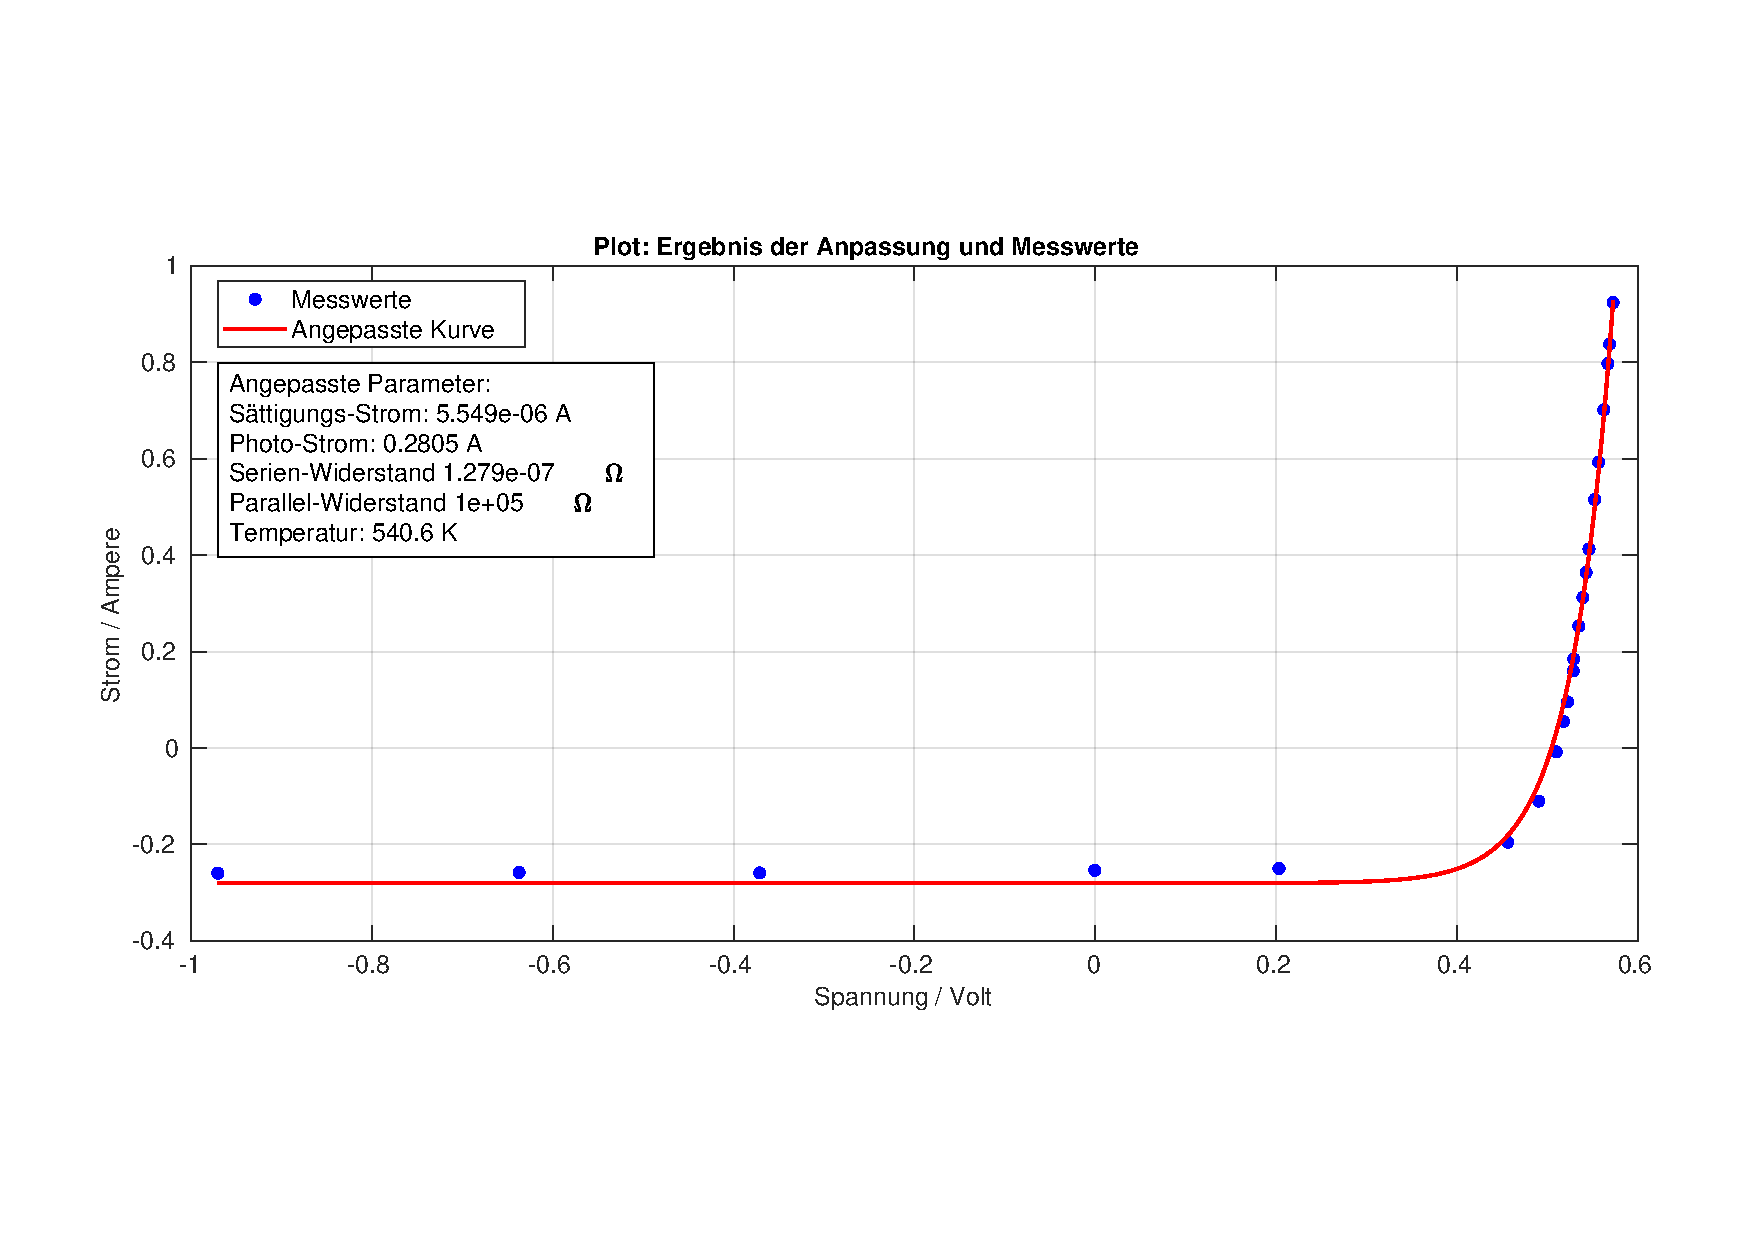
\includegraphics[width = \linewidth]{Bilder/SiMulti130Plot.pdf}
    \caption{Gefittete Schockley-Gleichung an das Mono-Si-Modul bei 130V}
\end{figure}
\begin{figure}[ht]
    \centering
    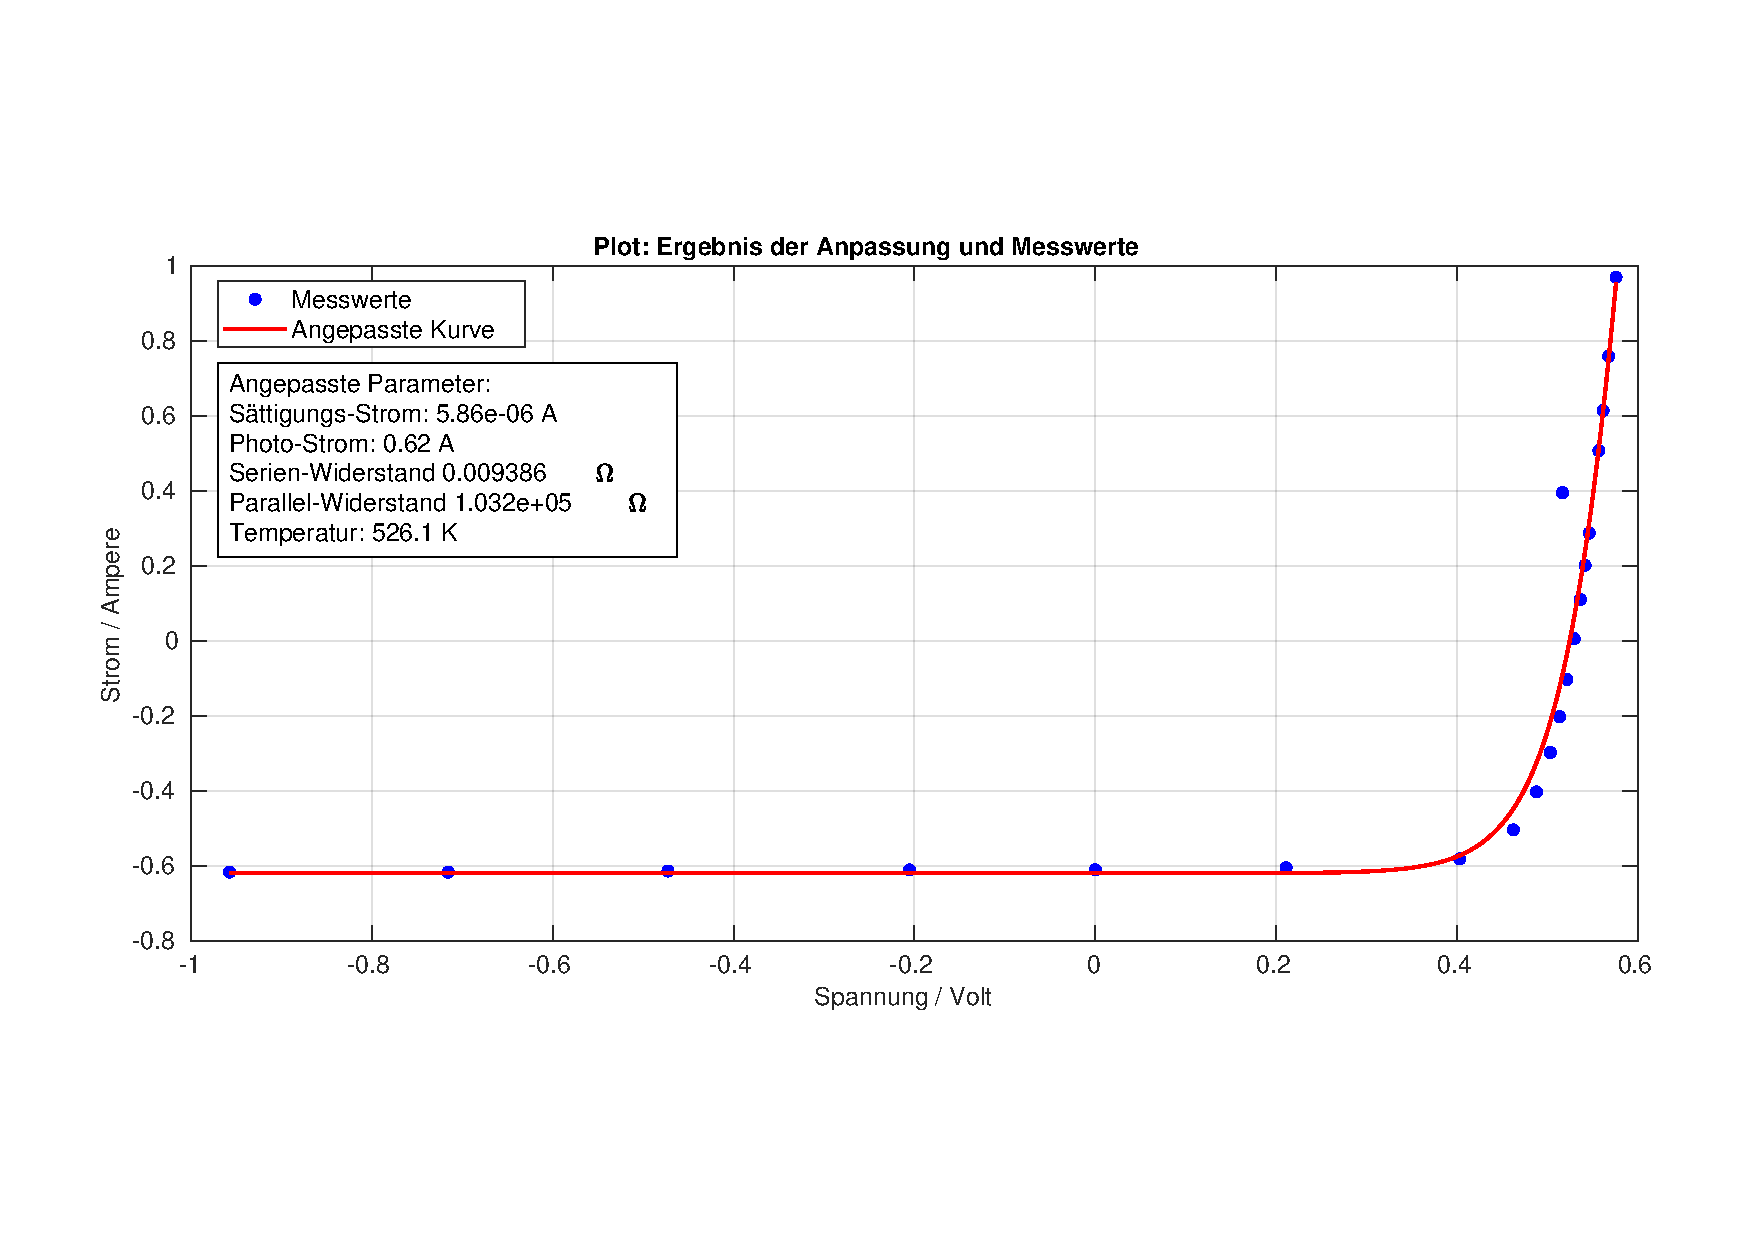
\includegraphics[width = \linewidth]{Bilder/SiMulti180Plot.pdf}
    \caption{Gefittete Schockley-Gleichung an das Mono-Si-Modul bei 130V}
\end{figure}
\begin{figure}[ht]
    \centering
    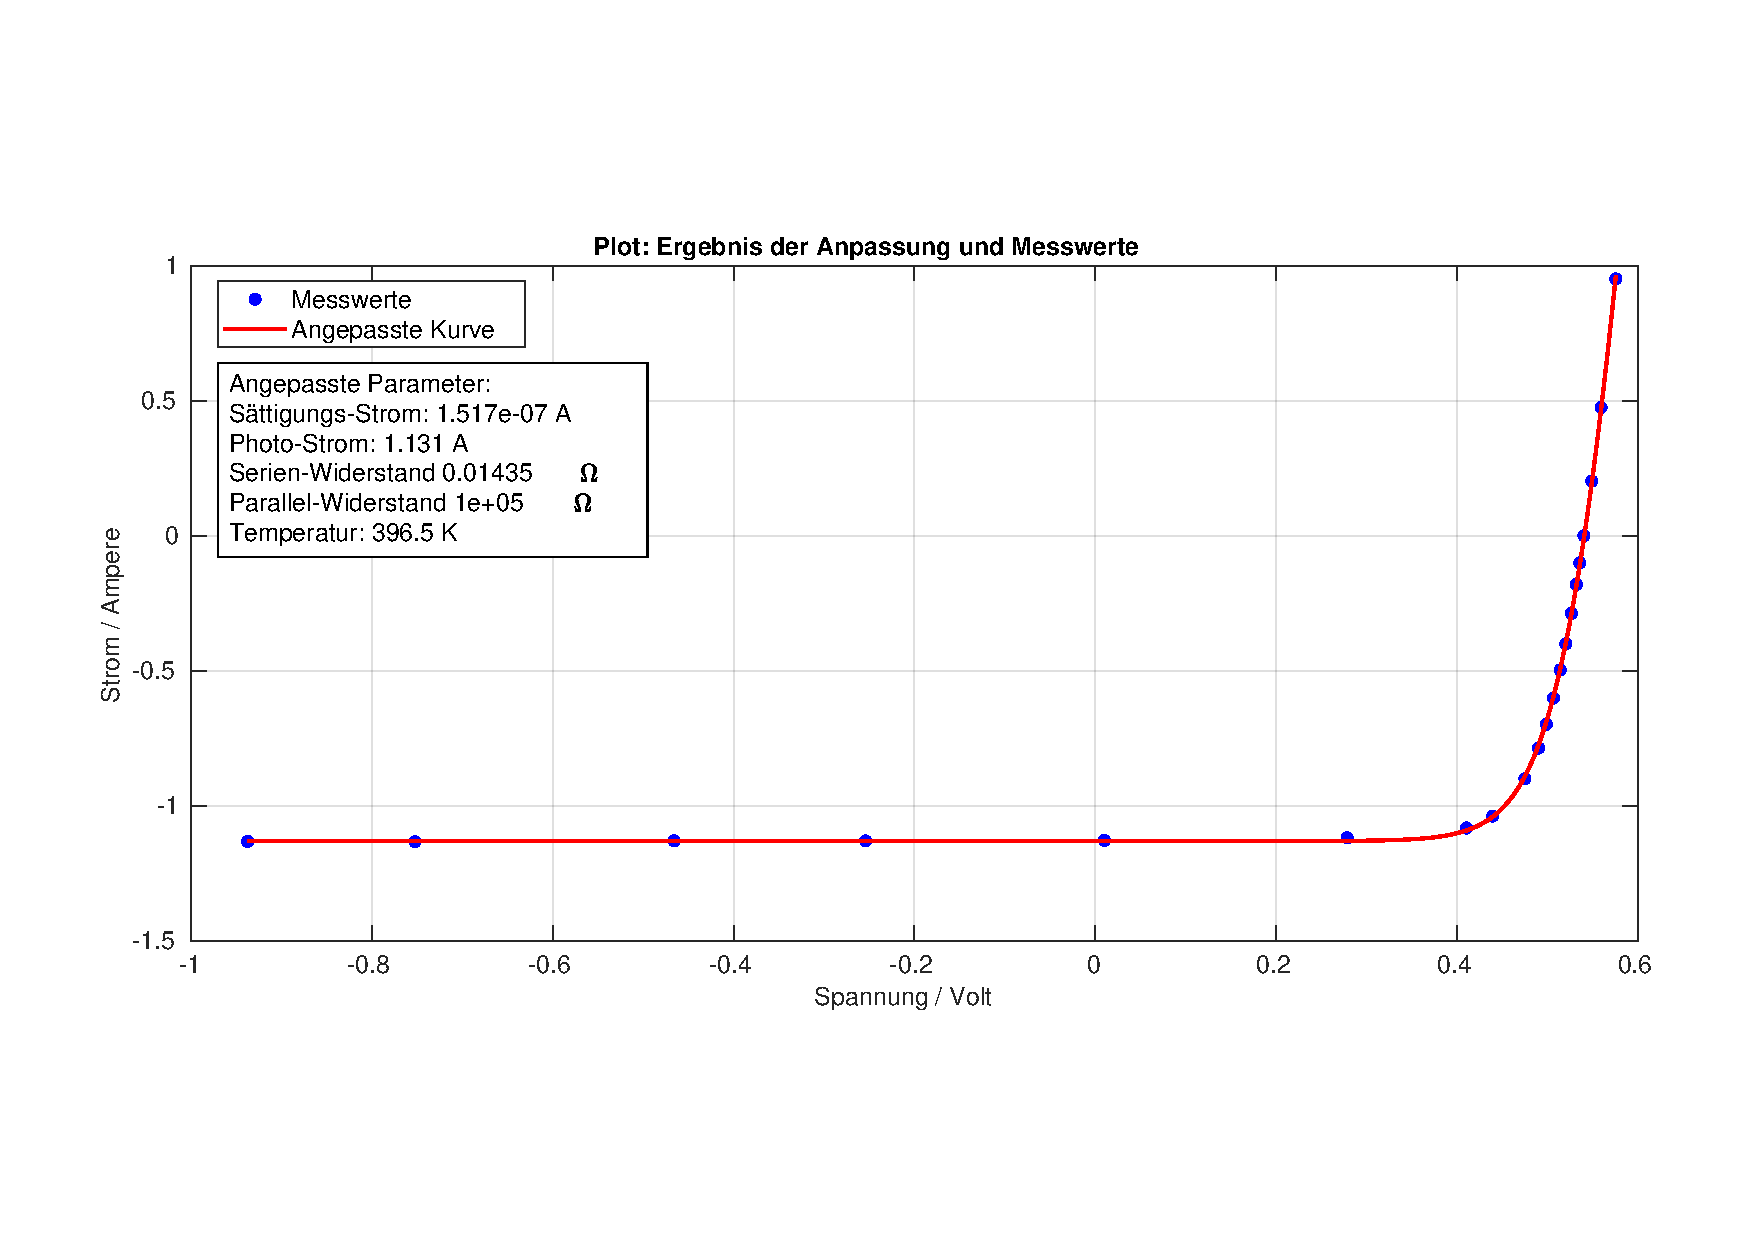
\includegraphics[width = \linewidth]{Bilder/SiMulti230Plot.pdf}
    \caption{Gefittete Schockley-Gleichung an das Mono-Si-Modul bei 130V}
\end{figure}
\begin{figure}[ht]
    \centering
    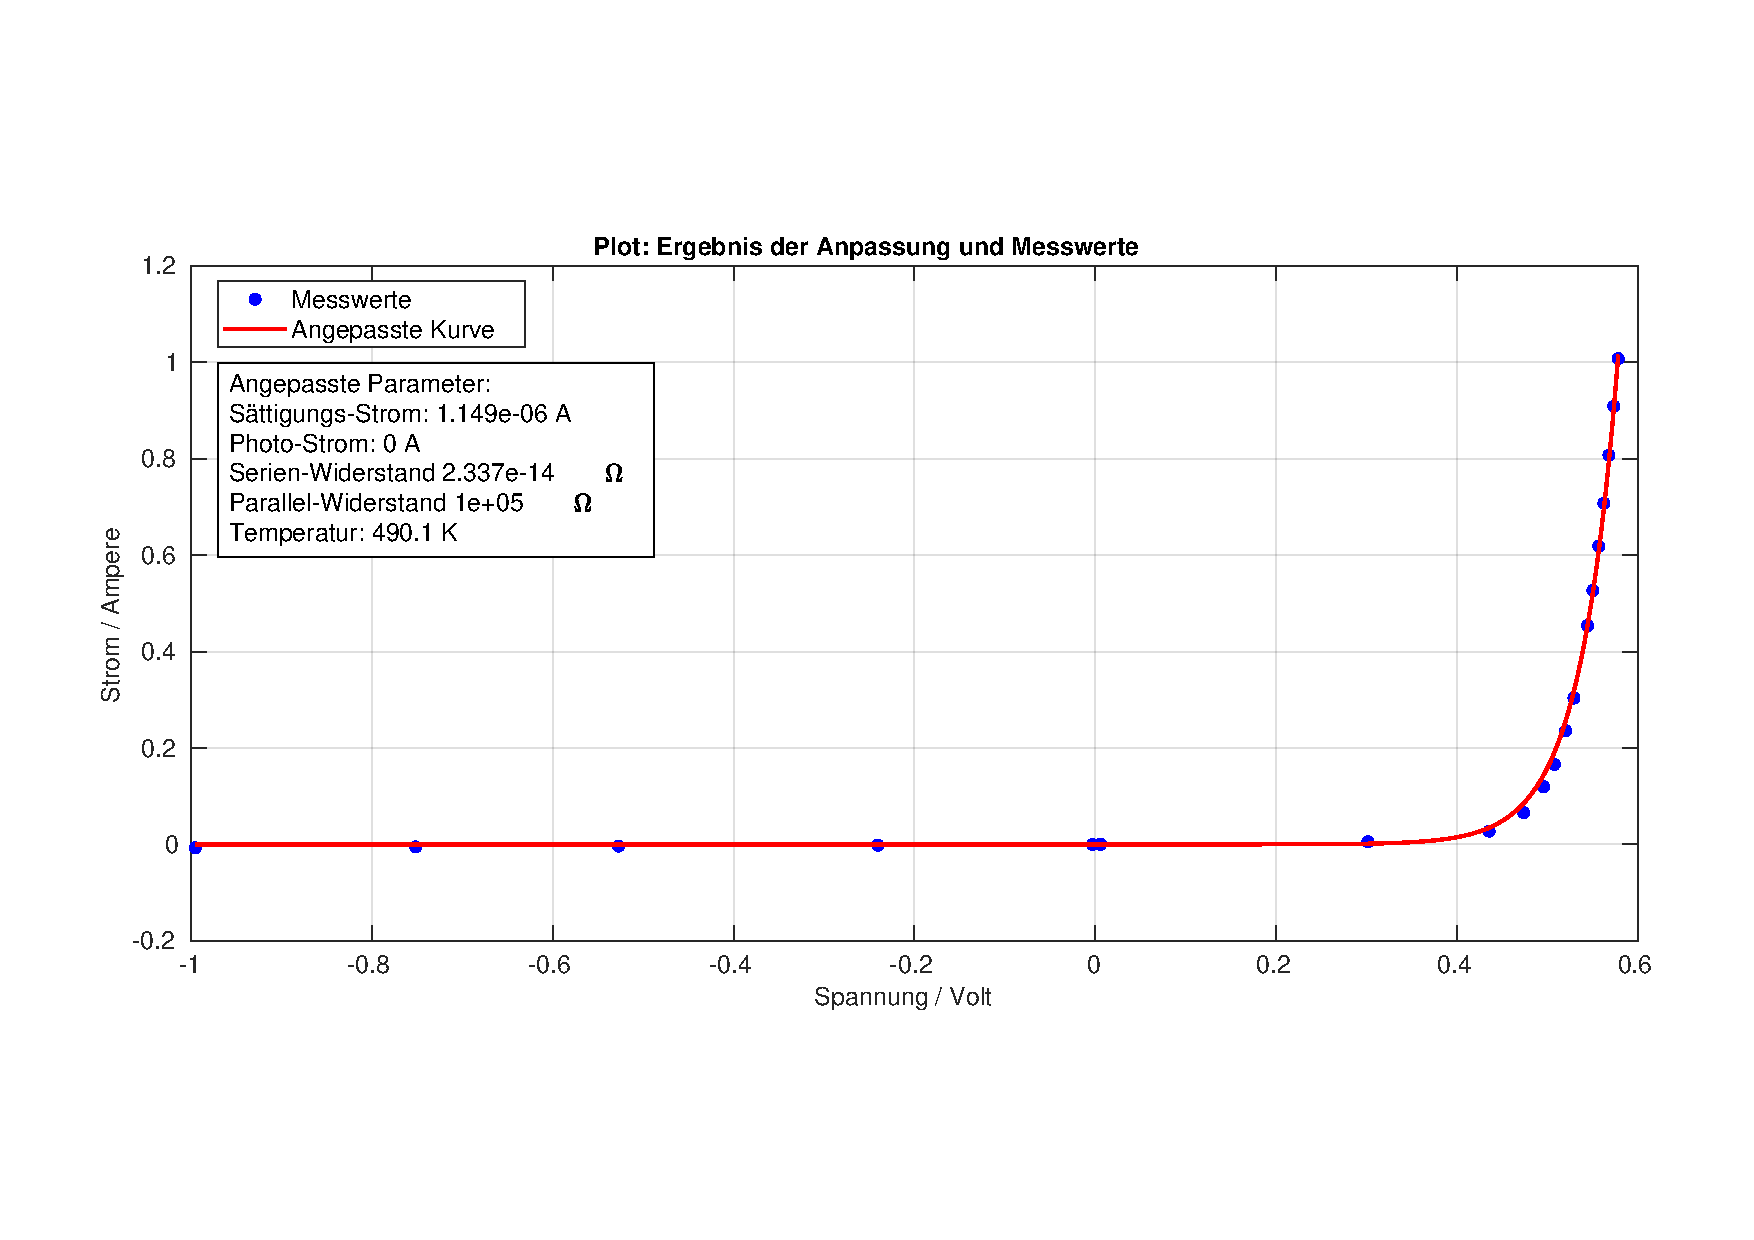
\includegraphics[width = \linewidth]{Bilder/SiMultiDunkelPlot.pdf}
    \caption{Gefittete Schockley-Gleichung an das Mono-Si-Modul bei 130V}
\end{figure}
\clearpage

\section{Wirkungsgrad}
\label{section:AnhangWirkungsgrad}

\begin{figure}[ht]
    \centering
    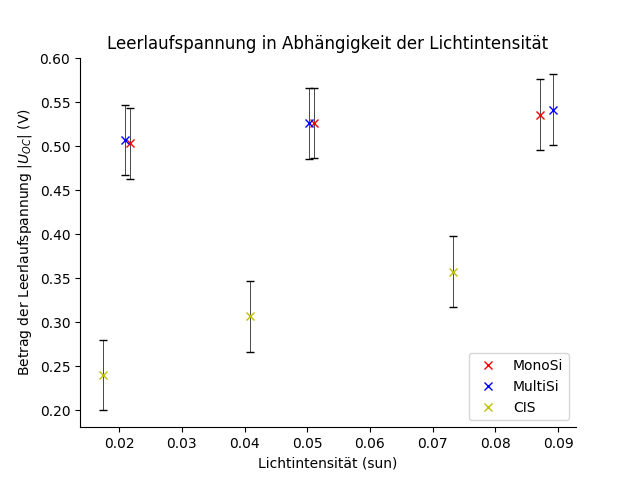
\includegraphics[width = \linewidth]{Bilder/PlotLeerlaufspannugnInt.png}
    \caption{Leerlaufspannung in Abhängigkeit der Lichtintensität}
\end{figure}

\begin{figure}[ht]
    \centering
    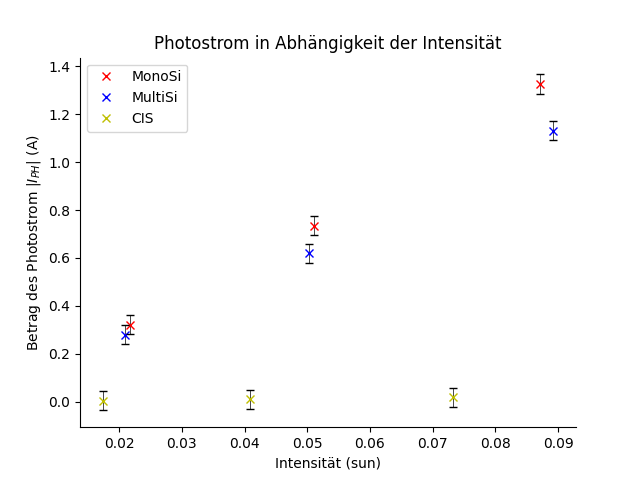
\includegraphics[width = \linewidth]{Bilder/PlotPhotostromInt.png}
    \caption{Photostrom in Abhängigkeit der Lichtintensität}

\end{figure}

\begin{figure}[ht]
    \centering
    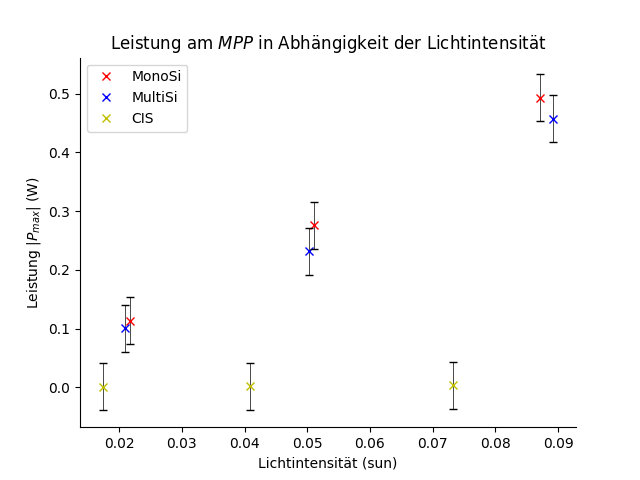
\includegraphics[width = \linewidth]{Bilder/PlotPMAXInt.png}
    \caption{Maximale Leistung $P_{Max}$ in Abhängigkeit der Lichtintensität}  
\end{figure}

\begin{figure}[ht]
    \centering
    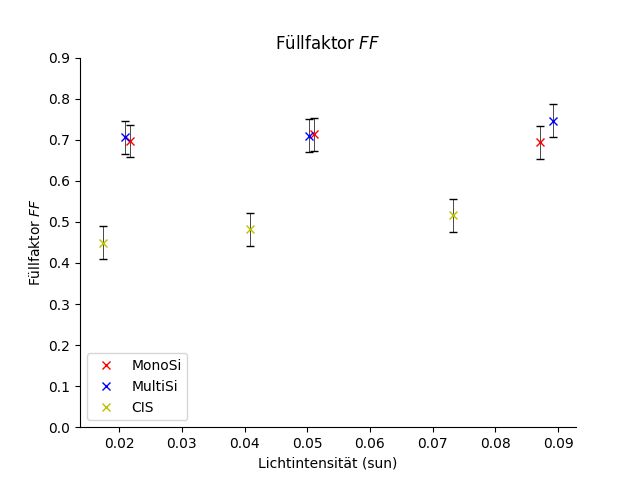
\includegraphics[width = \linewidth]{Bilder/PlotFFInt.png}
    \caption{Füllfaktor $FF$ in Abhängigkeit der Lichtintensität}  
\end{figure}
